\makeatletter
\def\input@path{{../styles/}{../../styles/}{../../../styles/}{../}{../../}{../../../}}
\makeatother


\documentclass{ee102_pset}
% macros.tex - Course meta information
\renewcommand{\course}{EE 102}
\renewcommand{\coursetitle}{Signal Processing and Linear Systems}
\renewcommand{\instructor}{Ayush Pandey}
\renewcommand{\semester}{Fall}
\renewcommand{\year}{2025}
\renewcommand{\shorttitle}{Week 1: Introduction to Signals}
% Use \renewcommand to avoid 'already defined' errors

% The following packages can be found on http:\\www.ctan.org
% \usepackage{graphics} % for pdf, bitmapped graphics files
%\usepackage{epsfig} % for postscript graphics files
%\usepackage{mathptmx} % assumes new font selection scheme installed
%\usepackage{times} % assumes new font selection scheme installed
\usepackage{amsmath} % assumes amsmath package installed
\usepackage{amssymb,mathtools}  % assumes amsmath package installed
\usepackage{xcolor}
\usepackage{pgfplots,subcaption}
\usepackage[hidelinks]{hyperref}
\usepackage{verbatim}
\usepackage{graphicx}
\usepackage{listings}

% -------- listings (Python) ----------
\lstdefinestyle{py}{
  language=Python,
  basicstyle=\ttfamily\small,
  keywordstyle=\color{blue!60!black}\bfseries,
  commentstyle=\color{green!40!black},
  stringstyle=\color{orange!60!black},
  showstringspaces=false,
  columns=fullflexible,
  frame=single,
  framerule=0.3pt,
  numbers=left,
  numberstyle=\tiny,
  xleftmargin=1em,
  tabsize=2,
  breaklines=true,
}
\usepackage[american]{circuitikz}
\usepackage{tikz}
\usepackage{caption}    
\usepackage{lscape}
\usepackage{soul}
\usepackage{tikz}
\usetikzlibrary{calc,angles,quotes,arrows.meta}

\usepackage{hyperref}
\hypersetup{
    colorlinks=true,
    linkcolor=blue,
    filecolor=magenta,      
    urlcolor=blue,
    pdftitle={week1_notes},
    pdfpagemode=FullScreen,
}
%\usepackage{float} 

%\usepackage[demo]{graphicx}
\pgfplotsset{compat=1.18}
% \usepgfplotslibrary{fillbetween}

\newsavebox{\measurebox}

\let\proof\relax\let\endproof\relax


\newcommand{\norm}[1]{\left\lVert#1\right\rVert}
\def\abs#1{\left\lvert#1\right\rvert}
\let\proof\relax
\let\endproof\relax
\usepackage{amsthm}
\usepackage{accents}
\usepackage{relsize}
\newcommand{\ubar}[1]{\underaccent{\bar}{#1}}
\newtheorem{theorem}{Theorem}
\newtheorem{corollary}{Corollary}[theorem]
\newtheorem{lemma}{Lemma}
\newtheorem{proposition}{Proposition}
\newtheorem{statement}{Statement}

\theoremstyle{definition}
\newtheorem{definition}{Definition}
 
\theoremstyle{remark}
\newtheorem*{remark}{Remark}
\theoremstyle{remark}
\newtheorem*{claim}{Claim}
\setlength{\parindent}{0cm}
\newenvironment{nalign}{
    \begin{equation}
    \begin{aligned}
}{
    \end{aligned}
    \end{equation}
    \ignorespacesafterend
}


% Assignment info
\author{\rule{3cm}{0.4pt}} % Name placeholder
\submitdate{\rule{3cm}{0.4pt}} % Submission date placeholder
\problemset{Homework \#6: Fourier Series}
\renewcommand{\duedate}{October 13, 2025}
\shorttitle{Homework \#6}

\begin{document}
\problem{1}
Consider the RC circuit example in previous problem sets and use its impulse response for this problem. For each of the input signals below, find the Fourier series representation of the output signal:

\problempart[20 points] A train of impulses:
\[
x(t) = \sum_{n=-\infty}^{\infty} \delta(t - n)
\]

Hint: You can find the Fourier series representation of the input signal and then use the property of LTI systems that relates the Fourier series coefficients of the input and output signals.
\problempart[20 points] A square wave of amplitude 1 sketched below in Figure~\ref{fig:square_wave}. 
\begin{figure}[h]
  \centering
  \begin{tikzpicture}[x=1.2cm,y=1.2cm,line cap=round]
  \pgfmathsetmacro{\H}{0.8}    % pulse height
  \pgfmathsetmacro{\W}{0.5}    % pulse width
  \pgfmathsetmacro{\hh}{0.5*\W}

  % axis
  \draw[->] (-3.6,0)--(4.6,0) node[below] {$t$};

  % pulses centered at integers
  \foreach \n in {-3,-2,-1,0,1,2,3,4}{
    \draw (\n-\hh,0) -- (\n-\hh,\H) -- (\n+\hh,\H) -- (\n+\hh,0);
  }

  % integer ticks and labels
  \foreach \n in {-3,-2,-1,0,1,2,3,4}{
    \draw (\n,0) -- ++(0,-0.06) node[below=2pt] {\small \n};
  }

  % ellipses at ends
  \node at (-3.9,0.58) {$\cdots$};
  \node at ( 4.0,0.58) {$\cdots$};

  % label x(t) over the n=0 pulse
  \draw[->] (0,\H-0.77) -- (0,\H+0.45);
  \node at (0,\H+0.75) {$x(t)$};

  % show width = 1/2 above the pulse at t=1
  \draw[<->] (1-\hh,\H+0.25) -- (1+\hh,\H+0.25)
    node[midway,fill=white,inner sep=1pt] {$\tfrac{1}{2}$};
\end{tikzpicture}
\caption{A square wave of amplitude $A$ and period $T=1$.}
\label{fig:square_wave}


\end{figure}

Hint: One period of the signal that is sketched above is \[
x(t) = \begin{cases}
1, & -\tfrac{1}{4} \le t \le \tfrac{1}{4},\\
0, & -\tfrac{1}{2} \le t < -\tfrac{1}{4},\\
0, & \tfrac{1}{4} < t \le \tfrac{1}{2}.
\end{cases}
\]
So, one possible time period is from $-\tfrac{1}{2}$ to $\tfrac{1}{2}$.
\problempart[20 points] The $x(t)$ above in part (b) models a PWM signal that drives a motor at a fixed duty cycle. As you engineer your system, you realized that you need double the speed of the motor. For this new PWM signal, sketch the signal and use the answer from the previous part along with properties of LTI systems to find the Fourier series representation of the output signal.

Hint: You can use the time-scaling property to solve this problem. Then use the previous results and properties of the Fourier series to get the final answer. So, you don't need to compute the Fourier series from scratch!

\problempart[10 points] Write Python/MATLAB code to implement the signals in (b) and (c). Compute the outputs, the Fourier series representations, and plot the magnitude spectra of the outputs. Validate your results using these simulations. 

\problem{2}
Compute the Fourier series representation of the following signals. For each part, if you consider only the first $N$ terms of the Fourier series, compute the error energy in the representation for $N=1,2,3,4$. You are allowed to use computer programs for computations, if it helps.

\problempart[15 points] A triangular signal with time period = 1. The sketch below in Figure~\ref{fig:problem2}A shows the signal for one time period from 0 to 1. The signal repeats itself periodically from 1 to 2, 2 to 3, and so on (and also for negative time, so you get a periodic signal).

Hint: This is only one part of the signal you worked on in the reading assignment. Use the results from that problem to get the Fourier series representation of this signal. 
\problempart[15 points] 
A rectangular signal sketched below in Figure~\ref{fig:problem2}B for one time period from 0 to 2. The time period of this signal is 2. The signal is 1 from 0 to 1 and 0 from 1 to 2. The signal repeats itself periodically for all time.

\begin{figure}[h]
\centering
  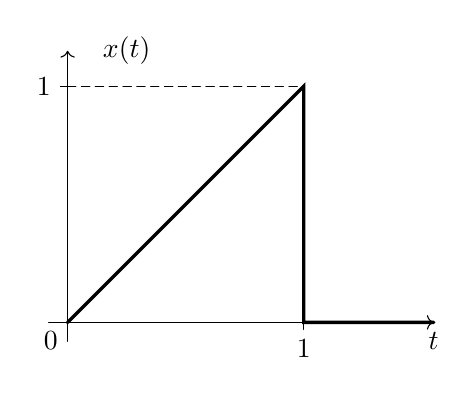
\begin{tikzpicture}[x=3.0cm,y=3.0cm,line cap=round]
\def\R{1.55}  % right extent
% axes
\draw[->] (-0.08,0)--(\R,0) node[below] {$t$};
\draw[->] (0,-0.08)--(0,1.15);
% ticks
\draw (0,1) -- ++(-0.03,0) node[left] {1};
\draw (1,0) -- ++(0,-0.03) node[below] {1};
\node[below left] at (0,0) {0};
% signal x(t): ramp on [0,1], drop, then 0
\draw[very thick] (0,0) -- (1,1) -- (1,0) -- (\R,0);
% guide at y=1
\draw[densely dashed] (0,1) -- (1,1);
% label
\node[above] at (0.25,1.05) {$x(t)$};
\end{tikzpicture}
\hspace{1.2cm}
% Figure (b): y(t)
\begin{tikzpicture}[x=3.0cm,y=3.0cm,line cap=round]
\def\R{2.5}
% axes
\draw[->] (-0.08,0)--(\R,0) node[below] {$t$};
\draw[->] (0,-0.08)--(0,1.15);
% ticks
\draw (0,1) -- ++(-0.03,0) node[left] {1};
\draw (1,0) -- ++(0,-0.03) node[below] {1};
\draw (2,0) -- ++(0,-0.03) node[below] {2};
\node[below left] at (0,0) {0};
% signal y(t): unit rectangle on [0,1]
\draw[very thick] (0,0) -- (0,1) -- (1,1) -- (1,0) -- (\R,0);
% label
\node[above] at (0.18,1.05) {$y(t)$};
\end{tikzpicture}
\caption{(a) A triangular signal $x(t)$ and (b) a rectangular signal $y(t)$.}
\label{fig:problem2}
\end{figure}

\end{document}
